\documentclass[12pt,a4paper]{article}
\usepackage[utf8]{inputenc}
\usepackage[vietnamese]{babel}
\usepackage{amsmath, amssymb}
\usepackage{graphicx}
\usepackage{geometry}
\geometry{a4paper, margin=2cm, headheight=15pt}
\usepackage{tabularx}
\usepackage{booktabs}
\usepackage[table]{xcolor}
\usepackage{titlesec}
\usepackage{fancyhdr}
\usepackage{mdframed}
\usepackage{systeme}
\usepackage{tcolorbox}
\usepackage{listings}
\usepackage{longtable}
\usepackage{multicol}
\usepackage{alltt}
\usepackage{minted}
\usepackage{enumitem}
\usepackage{float}
\usepackage{setspace}
\usepackage{xcolor} % Gói hỗ trợ màu sắc
\usepackage{soul}   % Gói hỗ trợ highlight text
\onehalfspacing
\usepackage[colorlinks=true, linkcolor=primary, urlcolor=secondary, citecolor=primary]{hyperref}
\usepackage[export]{adjustbox}

% ===== ĐỊNH NGHĨA MÀU SẮC =====
\definecolor{primary}{RGB}{0, 82, 155}     % Xanh dương đậm
\definecolor{secondary}{RGB}{0, 128, 128}  % Xanh cổ vịt (Teal)
\definecolor{codebg}{RGB}{245, 245, 245}   % Xám nhạt cho block code

% ===== ĐỊNH DẠNG TIÊU ĐỀ =====
\titleformat{\section}
  {\normalfont\Large\bfseries\color{primary}}
  {\thesection.}
  {0.5em}
  {}
  [{\titlerule[1pt]}]

\titleformat{\subsection}
  {\normalfont\large\bfseries\color{secondary}}
  {\thesubsection.}
  {0.5em}
  {}

\titleformat{\subsubsection}
  {\normalfont\normalsize\bfseries\color{primary}}
  {}
  {0em}
  {}

% ===== ĐỊNH DẠNG HEADER & FOOTER =====
\pagestyle{fancy}
\fancyhf{}
\fancyhead[L]{\textit{\color{gray}Báo cáo môn Quy hoạch tuyến tính}}
\fancyhead[R]{\textit{\color{gray}Nhóm ConTraiMeowMeow}}
\fancyfoot[C]{\thepage}
\renewcommand{\headrulewidth}{0.4pt}
\renewcommand{\footrulewidth}{0.4pt}

% ===== ĐỊNH DẠNG BLOCK CODE (VERBATIM) =====
\surroundwithmdframed[
    backgroundcolor=codebg,
    hidealllines=true,
    roundcorner=5pt,
    innertopmargin=10pt,
    innerbottommargin=10pt,
    innerleftmargin=10pt
]{verbatim}

% ===== TÙY CHỈNH KHOẢNG CÁCH DÒNG BẢNG =====
\renewcommand{\arraystretch}{1.3}

\begin{document}

% ==================== TRANG BÌA ====================
\begin{titlepage}
    \centering
    \vspace*{0.4cm}
    {\large \textbf{ĐẠI HỌC QUỐC GIA THÀNH PHỐ HỒ CHÍ MINH}\par}
    {\large \textbf{TRƯỜNG ĐẠI HỌC KHOA HỌC TỰ NHIÊN}\par}
    {\large KHOA TOÁN – TIN HỌC\par}
    \vspace{0.2cm}
    ------------ $\square$ \& $\square$ ------------\par
    
    \vspace{1cm} % Đã giảm khoảng trắng
    
\includegraphics[width=3cm, valign=t]{Images/logo-hcmus.png}
    \hspace{2.6cm}
    
\includegraphics[width=2.4cm, valign=t]{Images/logo-math.png}\par
    
    \vspace{2cm} % Đã giảm khoảng trắng
    {\large \bfseries BÁO CÁO BÀI TẬP NHÓM\par}
    {\large \bfseries MÔN HỌC: QUY HOẠCH TUYẾN TÍNH\par}
    \vspace{1cm}
    {\LARGE \bfseries CHƯƠNG TRÌNH GIẢI BÀI TOÁN\\[0.2cm]
    QUY HOẠCH TUYẾN TÍNH TỔNG QUÁT\par}
    
    \vspace{1cm} % Đã giảm khoảng trắng
    \begin{flushleft}
        \centering
        \normalsize % Hạ cỡ chữ xuống mức chuẩn để vừa trang
        \renewcommand{\arraystretch}{1.2} % Giảm dãn dòng nhẹ
        \begin{tabular}{p{4.8cm} l}
            \textbf{Mã môn học:} & MTH10449 \\
            \textbf{Mã lớp học:} & 24TTH\_KDL2 \\
            \textbf{Giảng viên giảng dạy:} & PGS.TS. Nguyễn Lê Hoàng Anh \\
            \textbf{Giảng viên trợ giảng :} & ThS. Nguyễn Mạnh Trường Giang \\
            \textbf{Nhóm sinh viên:} & 
            % Bảng lồng nhau chứa danh sách sinh viên
            \begin{tabular}[t]{@{}l@{\hspace{1cm}}l@{}}
                Nguyễn Đăng Nhân & MSSV: 24280038 \\
                Lê Tự Phong & MSSV: 24280039 \\
                Trần Nguyên Hưng & MSSV: 24280048 \\
                Vương Thành Đạt & MSSV: 24280058 \\
                Trương Đình Hưng & MSSV: 24280068 \\
            \end{tabular} \\
            \textbf{Ngành:} & Khoa học dữ liệu (Khóa 24)\\
        \end{tabular}
    \end{flushleft}
    
    \vfill
    {\normalsize \textit{TP. Hồ Chí Minh, ngày 11 tháng 6 năm 2026}}
    \vspace*{0.4cm}
\end{titlepage}

% ==================== MỤC LỤC ====================
\newpage
\renewcommand{\contentsname}{\centering \color{primary} MỤC LỤC}
\tableofcontents

% ==================== NỘI DUNG CHÍNH ====================
\newpage
\section{LỜI MỞ ĐẦU}
\hspace{\parindent}
Trong chương trình đào tạo kỹ thuật và kinh tế, Quy hoạch tuyến tính là một trong những môn học nền tảng với tính ứng dụng thực tiễn vô cùng lớn, từ việc tối ưu hóa chuỗi cung ứng, lập kế hoạch sản xuất cho đến quản lý nguồn lực. Tuy nhiên, đối với sinh viên, việc nắm bắt và áp dụng thuật toán Đơn hình (Simplex) – công cụ chính để giải các bài toán này – thường gặp không ít khó khăn do tính trừu tượng và sự phức tạp trong các bước tính toán thủ công. 

Với mong muốn hỗ trợ người học tiếp cận môn học một cách trực quan, sinh động và hiệu quả hơn, nhóm chúng em đã thực hiện dự án xây dựng \textit{\textbf{“Phần mềm Giải bài toán Quy hoạch tuyến tính tổng quát”}}. Phần mềm không chỉ đơn thuần là công cụ tính toán, mà còn là một nền tảng hỗ trợ học tập, giúp người dùng theo dõi từng bước biến đổi của bảng đơn hình, từ đó hiểu rõ bản chất của thuật toán. Bên cạnh đó, tính năng trực quan hóa bài toán 2D/3D giúp người học hình dung được miền nghiệm hình học, một khía cạnh trực quan quan trọng mà các bộ giải chuyên nghiệp thường bỏ qua. 

Trong quá trình thực hiện dự án, nhóm đã nỗ lực vận dụng các kiến thức đã học về Python, Tkinter và thuật toán tối ưu hóa để hiện thực hóa những yêu cầu đề ra. Dù còn nhiều hạn chế về quy mô và tính năng so với các bộ giải thương mại, chúng em hy vọng sản phẩm này sẽ là một tài liệu học tập hữu ích. 

Báo cáo này sẽ trình bày chi tiết về quá trình xây dựng, cấu trúc, các giải thuật đã sử dụng, cũng như hướng dẫn sử dụng phần mềm. Nhóm rất mong nhận được những góp ý từ quý Thầy Cô để sản phẩm ngày càng hoàn thiện hơn.

\newpage
\section{TỔNG QUAN VỀ DỰ ÁN}
\subsection{Thông tin nhóm}
{\centering
    \small
    \setlength{\extrarowheight}{1pt}
    \begin{longtable}{|c|c|l|l|c|c|}
        \hline
        \rowcolor{primary}
        \textcolor{white}{\textbf{TT}} &
        \textcolor{white}{\textbf{MSSV}} &
        \textcolor{white}{\textbf{Họ và tên}} &
        \textcolor{white}{\textbf{Email}} &
        \textcolor{white}{\textbf{Vai trò}} &
        \textcolor{white}{\textbf{Đánh giá}} \\ \hline
        \endfirsthead
        \hline
        \rowcolor{primary}
        \textcolor{white}{\textbf{TT}} &
        \textcolor{white}{\textbf{MSSV}} &
        \textcolor{white}{\textbf{Họ và tên}} &
        \textcolor{white}{\textbf{Email}} &
        \textcolor{white}{\textbf{Vai trò}} &
        \textcolor{white}{\textbf{Đánh giá}} \\ \hline
        \endhead

        1 & 24280038 & Nguyễn Đăng Nhân
          & {\footnotesize 24280038@student.hcmus.edu.vn}
          & Nhóm trưởng & 100\%\\ \hline
        \multicolumn{6}{|p{\dimexpr\textwidth-2\tabcolsep-2\arrayrulewidth\relax}|}{%
        \cellcolor{blue!5}\textit{\textbf{Nhiệm vụ:} Tập trung toàn bộ vào Frontend (UI/UX); điều chỉnh lời giải cho chặt chẽ; tạo các chức năng hiển thị lời giải qua định dạng HTML và các bảng từ vựng. Chịu trách nhiệm sửa lỗi một số trường hợp đặc biệt (vô số nghiệm, không giới nội, xoay vòng) và hoàn thiện phần phụ lục (test cases) trong báo cáo.}} \\ \hline

        2 & 24280039 & Lê Tự Phong
          & {\footnotesize 24280039@student.hcmus.edu.vn}
          & Thành viên & 100\% \\ \hline
        \multicolumn{6}{|p{\dimexpr\textwidth-2\tabcolsep-2\arrayrulewidth\relax}|}{%
        \cellcolor{blue!5}\textit{\textbf{Nhiệm vụ:} Phối hợp xây dựng chức năng trực quan đồ thị 2D, 3D và chuẩn hóa, tối ưu lại để phù hợp với từng trường hợp đặc biệt. Xây dựng các trường hợp mẫu (ví dụ minh họa). Chỉnh sửa phần thuật toán xử lý trường hợp ràng buộc đẳng thức. Hỗ trợ chỉnh sửa báo cáo.}} \\ \hline

        3 & 24280048 & Trần Nguyên Hưng
          & {\footnotesize 24280048@student.hcmus.edu.vn}
          & Thành viên & 100\%\\ \hline
        \multicolumn{6}{|p{\dimexpr\textwidth-2\tabcolsep-2\arrayrulewidth\relax}|}{%
        \cellcolor{blue!5}\textit{\textbf{Nhiệm vụ:} Lập trình các tiện ích quản lý form nhập liệu (Xóa toàn bộ / Reset). Đảm nhận khâu kiểm thử chất lượng trên các kịch bản: nghiệm duy nhất, vô nghiệm, nghiệm không giới nội, vô số nghiệm \ldots Soạn chính phần nội dung báo cáo.}} \\ \hline

        4 & 24280058 & Vương Thành Đạt
          & {\footnotesize 24280058@student.hcmus.edu.vn}
          & Thành viên & 100\% \\ \hline
        \multicolumn{6}{|p{\dimexpr\textwidth-2\tabcolsep-2\arrayrulewidth\relax}|}{%
        \cellcolor{blue!5}\textit{\textbf{Nhiệm vụ:} Dựng toàn bộ kiến trúc ban đầu, hoàn thành nền tảng sơ khai của ứng dụng, phát triển các thuật toán Đơn hình cốt lõi cho bài toán quy hoạch tuyến tính. Xây dựng chức năng Xuất lời giải thành file \texttt{.txt} và Nhập/Xuất đề bài với file \texttt{.csv}. Tìm kiếm các ứng dụng giải bài toán Quy hoạch tuyến tính.}}\\ \hline

        5 & 24280068 & Trương Đình Hưng
          & {\footnotesize 24280068@student.hcmus.edu.vn}
          & Thành viên & 100\% \\ \hline
        \multicolumn{6}{|p{\dimexpr\textwidth-2\tabcolsep-2\arrayrulewidth\relax}|}{%
        \cellcolor{blue!5}\textit{\textbf{Nhiệm vụ:} Xây dựng chức năng trực quan đồ thị 3D và kiểm thử từng trường hợp đặc biệt. Xây dựng thuật toán chạy đa luồng và tính năng đề xuất cách giải phù hợp, giải bằng cách khác ứng với từng bài toán. Mở rộng thuật toán cho trường hợp biến tự do và soạn phần hướng dẫn sử dụng trong báo cáo.}} \\ \hline
    \end{longtable}
}

\subsection{Mục tiêu phần mềm}
Phần mềm được xây dựng nhằm mục tiêu giải và minh họa từng bước quá trình giải bài toán Quy hoạch tuyến tính (Linear Programming) tổng quát theo Phương pháp Đơn hình (Simplex Method), phục vụ nhu cầu học tập và giảng dạy.

\medskip
\noindent\textit{\textbf{Các mục tiêu cụ thể:}}
\begin{itemize}[label=\textcolor{secondary}{$\bullet$}, itemsep=1pt]
    \item Hỗ trợ người dùng nhập bài toán Quy hoạch tuyến tính tổng quát ($\min$ / $\max$, ràng buộc $\leq$/$\geq$/=, biến $\geq 0$/$\leq 0$/tự do) qua giao diện đồ họa trực quan. 
    \item Tự động chuẩn hóa bài toán về dạng chuẩn, xây dựng từ vựng và thực hiện thuật toán Đơn hình với giải thích chi tiết từng bước xoay. 
    \item Tự động lựa chọn phương pháp giải phù hợp (Dantzig / Bland và Hai pha) dựa trên cấu trúc bài toán, và hiển thị thuật toán đề xuất cho người dùng. 
    \item Xuất kết quả ra nhiều định dạng (văn bản TXT, HTML có công thức \LaTeX, CSV), cung cấp trực quan hóa hình học (2D và 3D) và các bảng từ vựng.
    \item Đóng vai trò công cụ hỗ trợ giảng dạy: giảng viên có thể dùng trực tiếp trên lớp để minh họa, sinh viên dùng để tự kiểm tra bài tập. 
\end{itemize}

\newpage
\section{CÁC CHỨC NĂNG VÀ THUẬT TOÁN}
Phần mềm được thiết kế với giao diện thân thiện, tập trung vào khả năng tương tác và hỗ trợ giải thuật chi tiết. Các chức năng chính bao gồm:

\subsubsection*{Nhập liệu:}
\begin{itemize}[label=\textcolor{secondary}{$\circ$}, itemsep=1pt]
    \item Nhập số biến (1–5) và số ràng buộc (1–10) qua khung thiết lập; bảng nhập liệu tự sinh. 
    \item Hỗ trợ ba loại dấu ràng buộc: $\leq$, $\geq$, =. 
    \item Hỗ trợ ba loại dấu biến: $\geq 0$, $\leq 0$, tự do. 
    \item Hỗ trợ nhập hệ số dạng phân số (ví dụ 1/2, 3/4) hoặc số thập phân; toàn bộ tính toán nội bộ dùng kiểu \texttt{Fraction} (số hữu tỉ chính xác tuyệt đối). 
    \item Nhập/xuất bài toán qua file CSV theo định dạng chuẩn riêng. 
    \item Tích hợp 9 bài toán mẫu (demo preset) sẵn có để điền tự động. 
\end{itemize}

\subsubsection*{Chuẩn hóa bài toán:}
\textit{Phần mềm thực hiện đầy đủ quy trình chuẩn hóa và hiển thị tường minh từng bước}
\begin{itemize}[label=\textcolor{secondary}{$\circ$}, itemsep=1pt]
    \item Biến $\leq 0$: thay $x_i = -y_i, y_i \geq 0$.
    \item Biến tự do: thay $x_i = a_i - b_i, a_i, b_i \geq 0$.
    \item Bài toán $\max$: nhân $(-1)$ vào hàm mục tiêu, đưa về dạng $\min$. 
    \item Ràng buộc $\geq$: nhân $(-1)$ vào cả 2 vế để đưa về dạng $\leq$. 
    \item Ràng buộc $=$: tách thành hai ràng buộc $\leq$ (hướng thuận và nghịch). 
    \item Thêm biến bù cho từng ràng buộc $\leq$ để xây dựng từ vựng xuất phát.
\end{itemize}

\subsubsection*{Các thuật toán:}
Phần mềm triển khai ba phương pháp, chạy đa luồng (multi-thread) để so sánh:

\begin{table}[h]
    \centering
    \rowcolors{1}{white}{blue!5}
    \begin{tabularx}{\textwidth}{|l|X|X|}
        \hline
        \rowcolor{primary}
        \textcolor{white}{\textbf{Thuật toán}} & \textcolor{white}{\textbf{Khi nào áp dụng}} & \textcolor{white}{\textbf{Ghi chú}} \\ \hline
        Phương pháp Dantzig & $b_i > 0$ với mọi $i$ & Chọn biến vào cơ sở có khả năng cải thiện hàm mục tiêu nhiều nhất ở mỗi bước pivot \\ \hline
        Phương pháp Bland & Tồn tại $b_i = 0$, có nguy cơ xoay vòng nếu giải bằng Dantzig & Chọn biến vào cơ sở có chỉ số nhỏ nhất trong các biến đủ điều kiện \\ \hline
        Phương pháp Hai pha & Tồn tại $b_i < 0$ & Tạo và giải một bài toán phụ để tìm nghiệm cơ sở khả thi ban đầu trước khi giải bài toán gốc bằng Dantzig \\ \hline
    \end{tabularx}
\end{table}

\textit{\textbf{Phần mềm tự động phát hiện và xử lý:}}
\begin{itemize}[label=\textcolor{secondary}{$-$}, itemsep=1pt]
    \item \textit{Xoay vòng (cycling):} trình bày lời giải bằng Dantzig để thấy được xoay vòng và đề xuất người dùng chuyển sang Bland; nếu phát hiện xoay vòng với bài toán Hai pha thì sau khi giải bằng Dantzig sẽ chuyển sang giải bằng Bland để hoàn thành bài toán.
    \item \textit{Suy biến (degeneracy):} đếm và thông báo số bước suy biến ($\theta = 0$). 
    \item \textit{Không giới nội (unbounded):} phát hiện khi không tìm được biến ra. 
    \item \textit{Vô số nghiệm (multiple optimal):} phát hiện khi có biến không cơ sở với hệ số 0 trên hàm mục tiêu; trình bày nghiệm tổng quát theo tham số.
    \item \textit{Vô nghiệm (infeasible):} phát hiện khi giá trị bổ trợ sau Pha 1 $x_0 > 0$. 
\end{itemize}

\subsubsection*{Hiển thị lời giải:}
\begin{itemize}[label=\textcolor{secondary}{$\circ$}, itemsep=1pt]
    \item In bài toán gốc và toàn bộ quá trình chuẩn hóa. 
    \item In từng bảng từ vựng trước và sau mỗi bước xoay, với highlight màu: cột biến vào (vàng nhạt), hàng biến ra (xanh lam nhạt), ô phần tử xoay (xanh đậm).
    \item Giải thích tường minh lý do chọn biến vào (Dantzig/Bland), bảng tỉ số $\theta$, phần tử xoay. 
    \item Kết luận cuối: trạng thái bài toán, giá trị tối ưu, nghiệm tối ưu (kể cả nghiệm tổng quát nếu vô số nghiệm). 
    \item Hiển thị khuyến nghị phương pháp phù hợp và cho phép chuyển đổi xem lời giải theo từng phương pháp. 
\end{itemize}

\subsubsection*{Xuất kết quả:}
\begin{itemize}[label=\textcolor{secondary}{$\circ$}, itemsep=1pt]
    \item Xuất \texttt{.txt}: nội dung toàn bộ lời giải dạng văn bản thuần. 
    \item Xuất \textbf{HTML}: trang web có định dạng đẹp với công thức \LaTeX (KaTeX), bảng từ vựng có màu highlight, thanh tiến trình, tự mở trình duyệt mặc định. 
    \item Xuất/Nhập \texttt{.csv}: lưu và tải lại bài toán (không phải lời giải). 
\end{itemize}

\subsubsection*{Trực quan hóa (Phương pháp hình học):}
\begin{itemize}[label=\textcolor{secondary}{$\circ$}]
    \item \textbf{2D (2 biến):} vẽ miền chấp nhận được, các đường ràng buộc, đường đồng mức hàm mục tiêu, đánh dấu các điểm tối ưu và hiển thị đường đi khi giải bằng Dantzig hoặc Bland. Hỗ trợ pan (kéo chuột) và zoom (lăn chuột / nút). 
    \item \textbf{3D (3 biến):} vẽ các mặt phẳng ràng buộc và vùng khả thi trong không gian 3 chiều. 
\end{itemize}

\subsubsection*{Hiện từ vựng từng bước:} Module \texttt{animator.py} cung cấp cửa sổ pop-up riêng, hiển thị bảng từ vựng Đơn hình dưới dạng bảng ô màu sắc (như trình chiếu slide), với nút điều hướng Trước/Sau, tự động highlight biến vào/ra/ô xoay ở từng bước. Hỗ trợ cả bài toán một pha và hai pha.

\section{HƯỚNG DẪN SỬ DỤNG}

\subsection{Cài đặt và chạy chương trình}

\noindent\textbf{Cách 1: Chạy file .exe đã đóng gói (dành cho người dùng)}\\
Tải file \href{https://drive.google.com/file/d/1MgmYg_NiuSky7lKlPjDzfYT9onzOd6Mu/view?usp=sharing}{\texttt{lp\_solver.exe}} và chạy trực tiếp - không cần cài Python hay bất kỳ thư viện nào.

\medskip
\noindent\textbf{Cách 2: Chạy từ mã nguồn (dành cho developer)}\\
Clone repository \url{https://github.com/vngthdat206/LinearProgrammingTool_byVC} về máy, sau đó cài đặt môi trường:

\textit{\textbf{Bước 1: Clone repository}}
\begin{verbatim}
git clone https://github.com/vngthdat206/LinearProgrammingTool_byVC
\end{verbatim}
Sử dụng lệnh sau để truy cập vào thư mục vừa tải về.
\begin{verbatim}
cd LinearProgrammingTool_byVC
\end{verbatim}

\textit{\textbf{Bước 2. (Khuyến nghị) Tạo môi trường ảo}}

\noindent Tạo môi trường ảo để quản lý thư viện riêng biệt cho dự án:
\begin{verbatim}
python -m venv .venv
\end{verbatim}
Sử dụng lệnh kích hoạt phù hợp với hệ điều hành:
\begin{verbatim}
# Windows
.venv\Scripts\activate
# macOS/Linux
source .venv/bin/activate
\end{verbatim}

\textit{\textbf{Bước 3: Cài đặt các gói cần thiết thông qua file \texttt{requirements.txt}}}
\begin{verbatim}
python -m pip install --upgrade pip
python -m pip install -r requirements.txt
\end{verbatim}

\textit{\textbf{Bước 4: Chạy ứng dụng}}
\begin{verbatim}
python main.py
\end{verbatim}

\textit{\textbf{Build lại \texttt{lp\_solver.exe} từ file cấu hình \texttt{main.spec}}}
\begin{verbatim}
pyinstaller --distpath . lp_solver.spec
\end{verbatim}
File output nằm ở thư mục hiện tại.

\subsection{Các bước thao tác}
Để giải một bài toán Quy hoạch tuyến tính, người dùng thực hiện theo quy trình 4 bước đơn giản dưới đây:

\textbf{Bước 1: Thiết lập bài toán}\\
Ở khung Thiết lập, chọn số biến (1–5) và số ràng buộc (1–10). Bảng nhập liệu tự cập nhật.

\begin{figure}[H] %
    \centering
    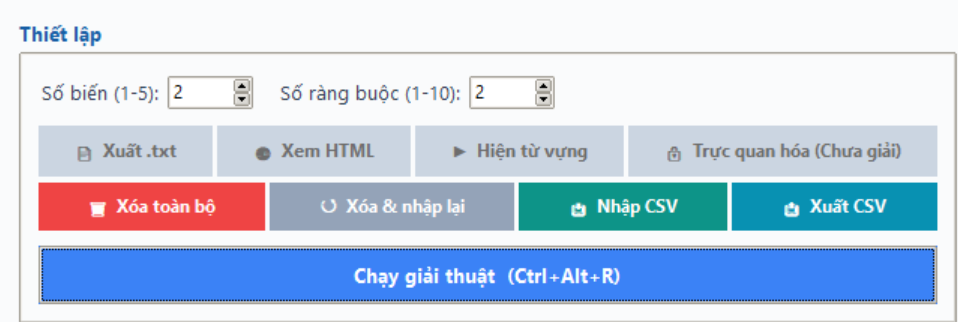
\includegraphics[width=0.75\textwidth]{Images/Buoc1.png}
    \caption{Chọn số biến và số ràng buộc}
    \label{fig:buoc1}
\end{figure}

\textbf{Bước 2: Nhập bài toán}\\
Trong khung Nhập bài toán:
\begin{itemize}[label=\textcolor{secondary}{$-$}, itemsep=1pt]
    \item Chọn kiểu bài toán: max hoặc min.
    \item Nhập hệ số hàm mục tiêu cho từng biến $x_1, x_2, \dots$
    \item Chọn dấu của từng biến ($\geq 0, \leq 0$, hoặc tự do).
    \item Nhập từng ràng buộc: các hệ số, dấu ($\leq/\geq/=$), và nhập số ở vế phải.
\end{itemize}
Có thể dùng phím Tab để chuyển giữa các ô, hoặc dùng cuộn chuột để xem toàn bộ bảng khi có nhiều ràng buộc.
\\
Ngoài ra có thể chọn \textbf{Nhập CSV} để nhập các bài toán đã được lưu trước đó, hoặc các bài toán mẫu (ở phần PHỤ LỤC).


\begin{figure}[H] %
    \centering
    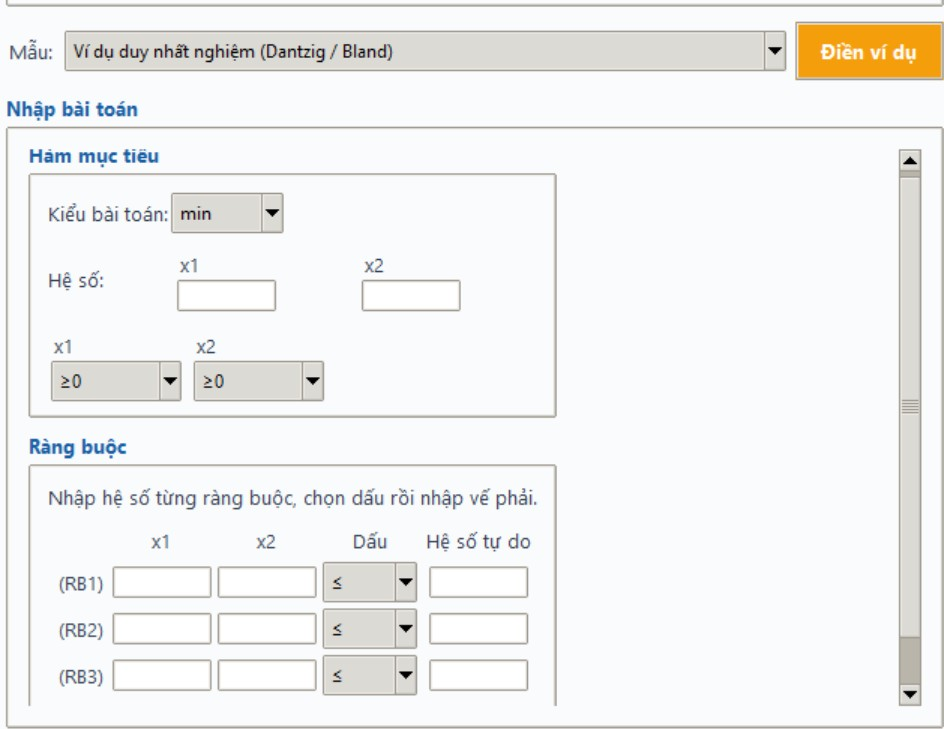
\includegraphics[width=0.75\textwidth]{Images/Buoc2.jpg}
    \caption{Nhập bài toán}
    \label{fig:buoc2}
\end{figure}


\noindent\textit{Mẹo:} Nhấn nút \textbf{Điền ví dụ} để tự động điền một trong 9 bài toán mẫu có sẵn, bao gồm các trường hợp: duy nhất nghiệm, vô số nghiệm, không giới nội, vô nghiệm, và xoay vòng. Hoặc nhập CSV với các mẫu test cases ở phụ lục, hoặc các file CSV đã được tải về trước đó (có định dạng phù hợp).

\medskip
\textbf{Bước 3: Chạy giải thuật}\\
Kiểm tra lại dữ liệu và Nhấn nút \textbf{Chạy giải thuật (Ctrl+Alt+R)}. Phần mềm sẽ:
\begin{itemize}[label=\textcolor{secondary}{$-$}, itemsep=1pt]
    \item Giải song song bằng cả Dantzig và Bland.
    \item Hiển thị khuyến nghị phương pháp phù hợp (Dantzig / Bland / Hai Pha) dựa trên cấu trúc bài toán.
    \item Hiển thị toàn bộ lời giải trong khung Lời giải bên phải.
\end{itemize}
\begin{figure}[H] %
    \centering
    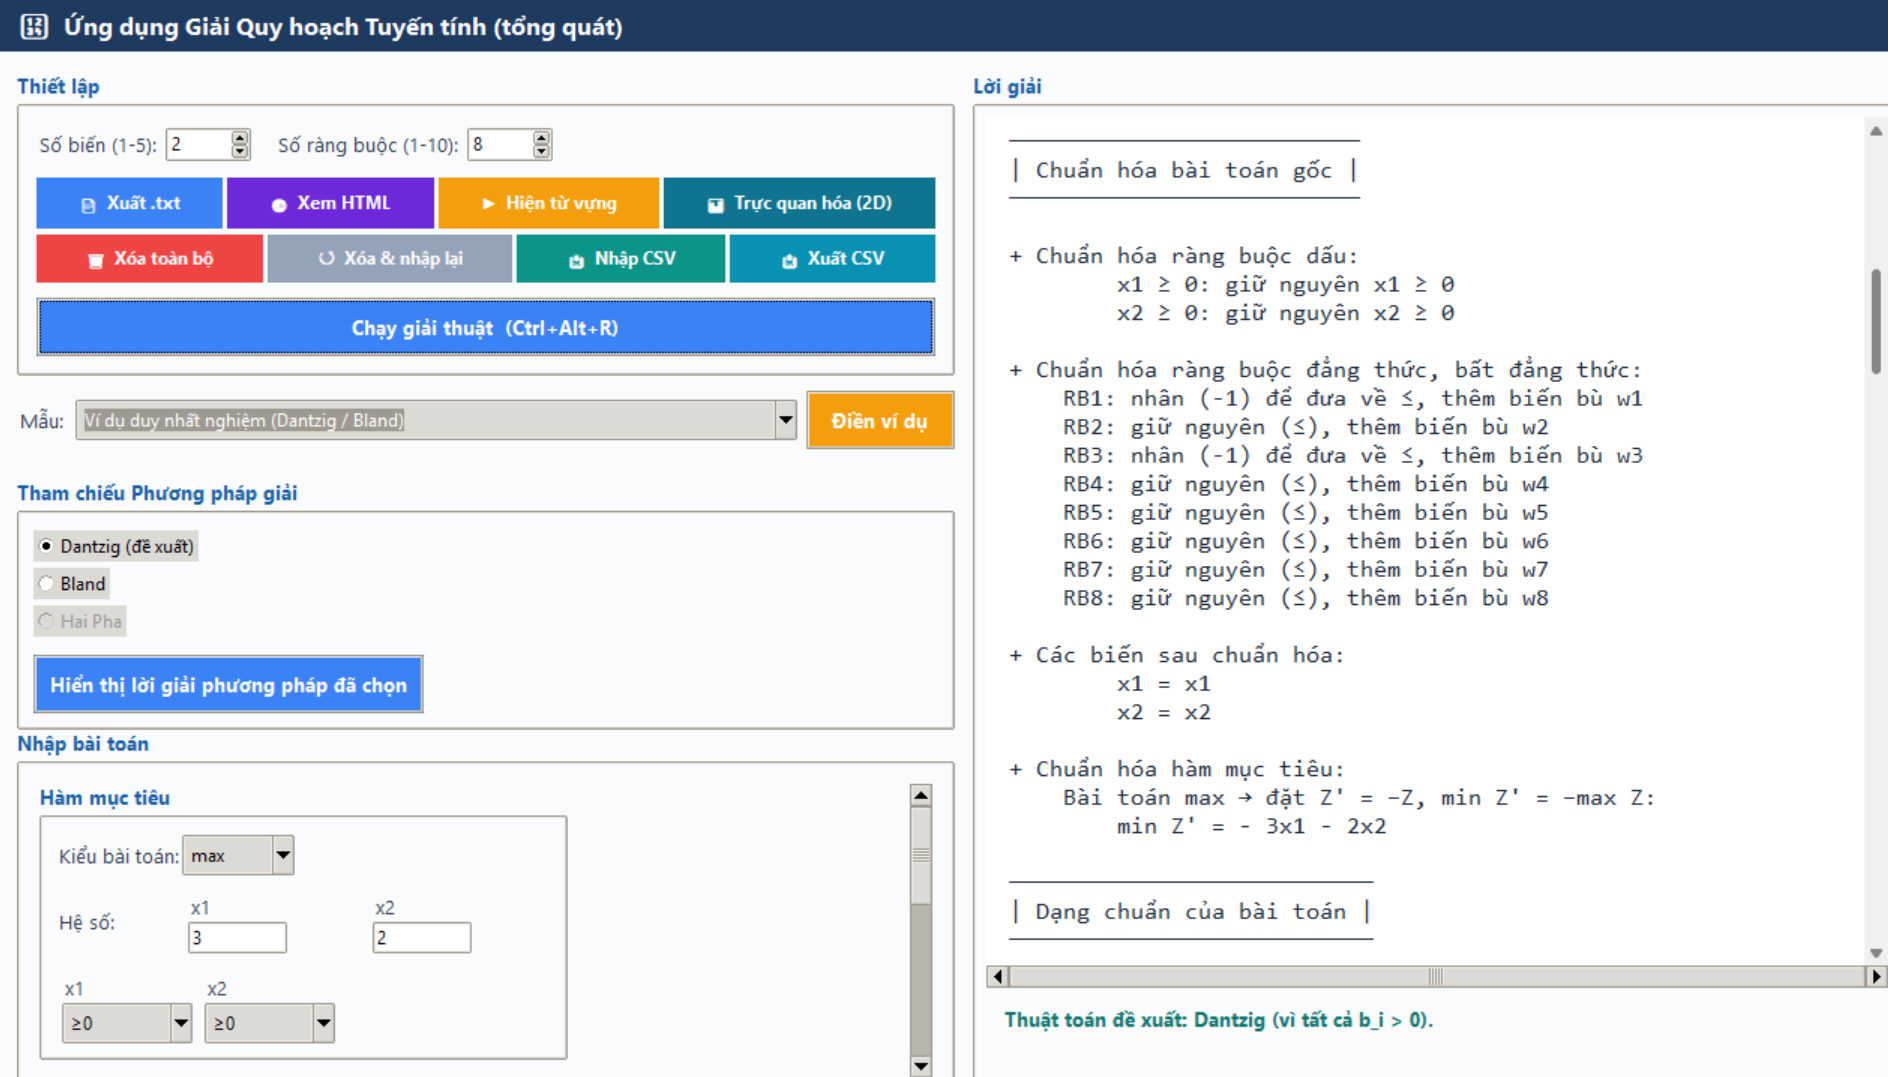
\includegraphics[width=0.75\textwidth]{Images/Buoc3.png}
    \caption{Hình ảnh sau khi chạy}
    \label{fig:buoc3}
\end{figure}

\begin{figure}[H] %
    \centering
    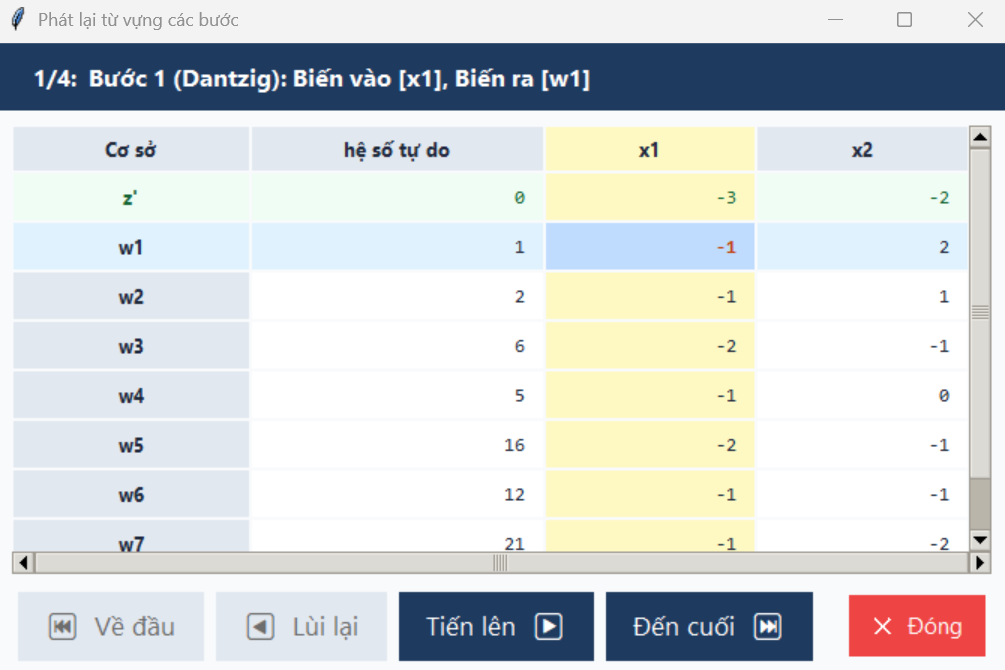
\includegraphics[width=0.75\textwidth]{Images/tuvung.png}
    \caption{Hình ảnh từ vựng thông qua nút Hiện từ vựng}
    \label{fig:buoc3s}
\end{figure}


\textbf{Bước 4: Xem lời giải theo phương pháp khác}\\
Ở khung Tham chiếu Phương pháp giải, chọn phương pháp muốn xem (Dantzig / Bland / Hai Pha) rồi nhấn \textbf{Hiển thị lời giải phương pháp đã chọn}. Các phương pháp không phù hợp với bài toán hiện tại sẽ bị mờ.


\begin{figure}[H] %
    \centering
    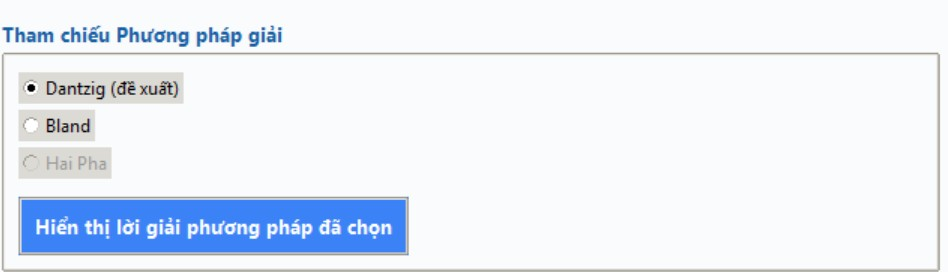
\includegraphics[width=0.75\textwidth]{Images/Buoc4.jpg}
    \caption{Hình ảnh khung tham chiếu phương pháp giải}
    \label{fig:buoc4}
\end{figure}

\textbf{Bước 5 – Xuất kết quả}\\
Sau khi có lời giải, các nút sau được kích hoạt:
\begin{itemize}[label=\textcolor{secondary}{$-$}, itemsep=1pt]
    \item \textbf{Xuất .txt:} lưu lời giải ra file văn bản.
    \item \textbf{Xem HTML:} HTML có công thức đẹp và mở trong trình duyệt.
    \item \textbf{Hiện từ vựng:} mở cửa sổ Animator để xem lại từng bước xoay.
    \item \textbf{Trực quan hóa:} mở đồ thị 2D (2 biến) hoặc 3D (3 biến).
\end{itemize}
Ngoài ra để lưu bài toán lại thì có thể chọn \textbf{Xuất CSV}: lưu bài toán hiện tại ra file CSV để dùng lại sau.


\begin{figure}[H] %
    \centering
    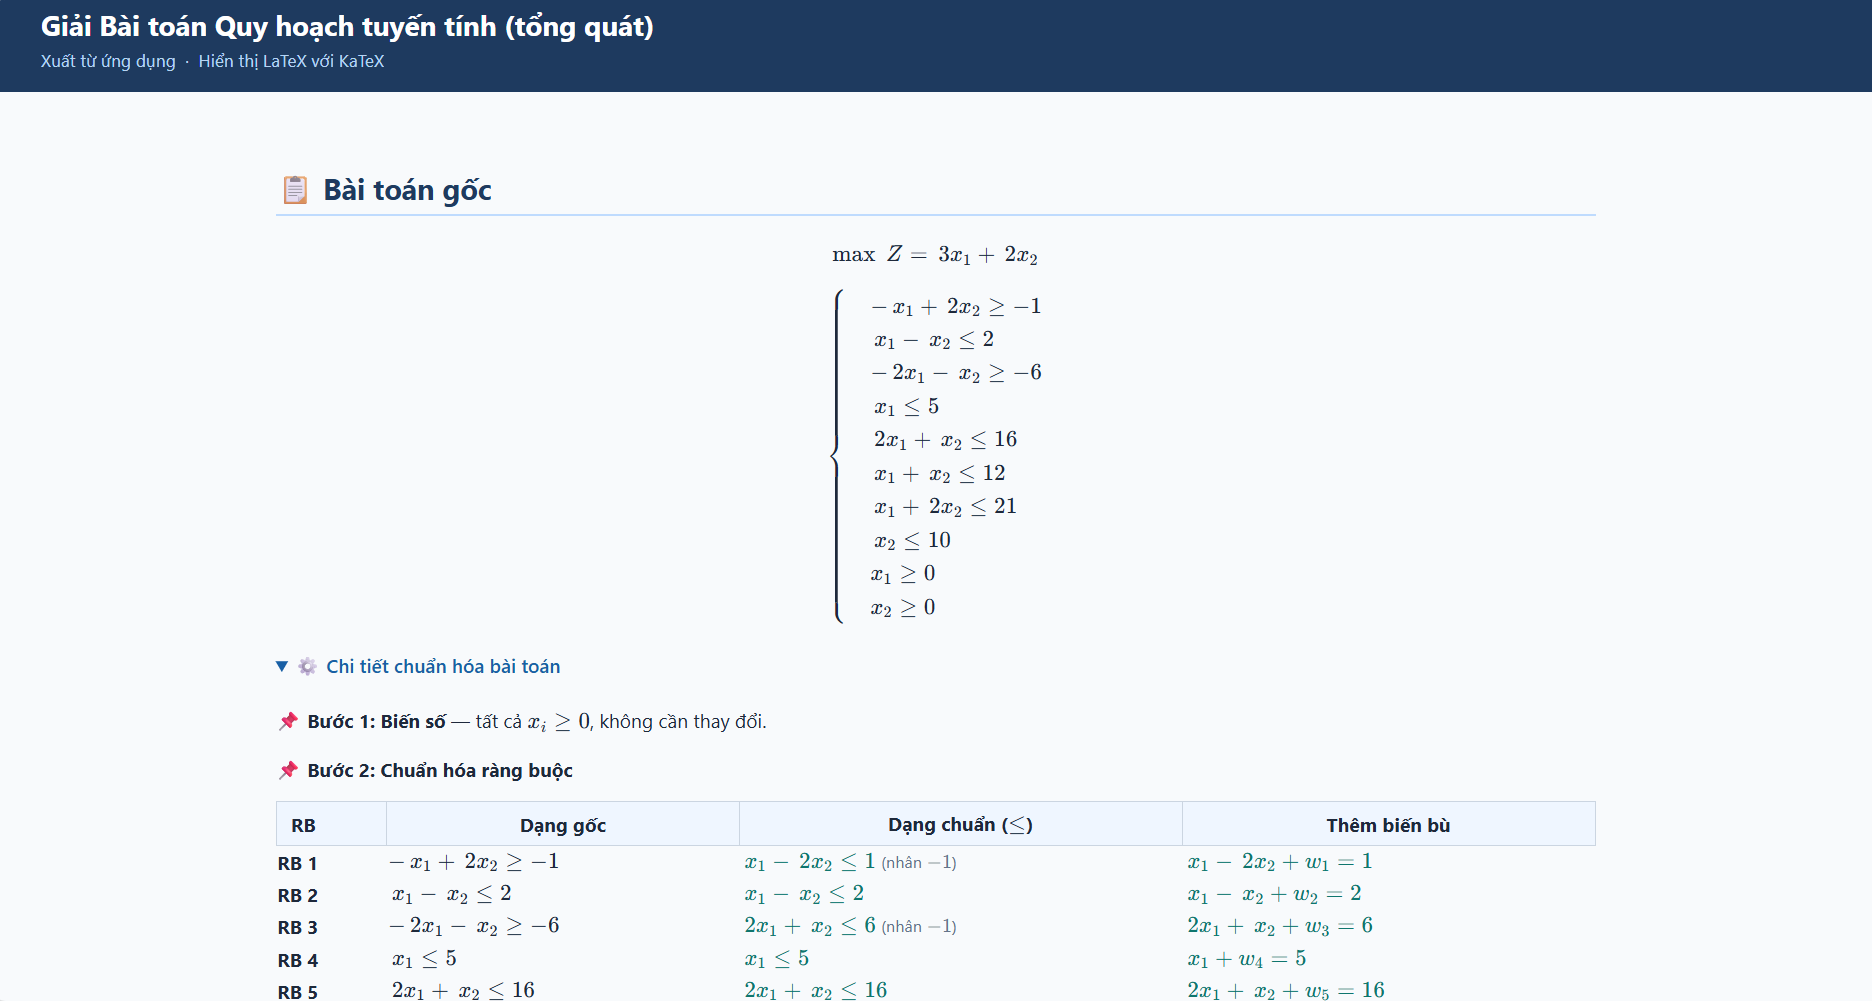
\includegraphics[width=0.75\textwidth]{Images/HTML.png}
    \caption{Hình ảnh xuất kết quả ra HTML}
    \label{fig:buoc5}
\end{figure}


\begin{figure}[H] %
    \centering
    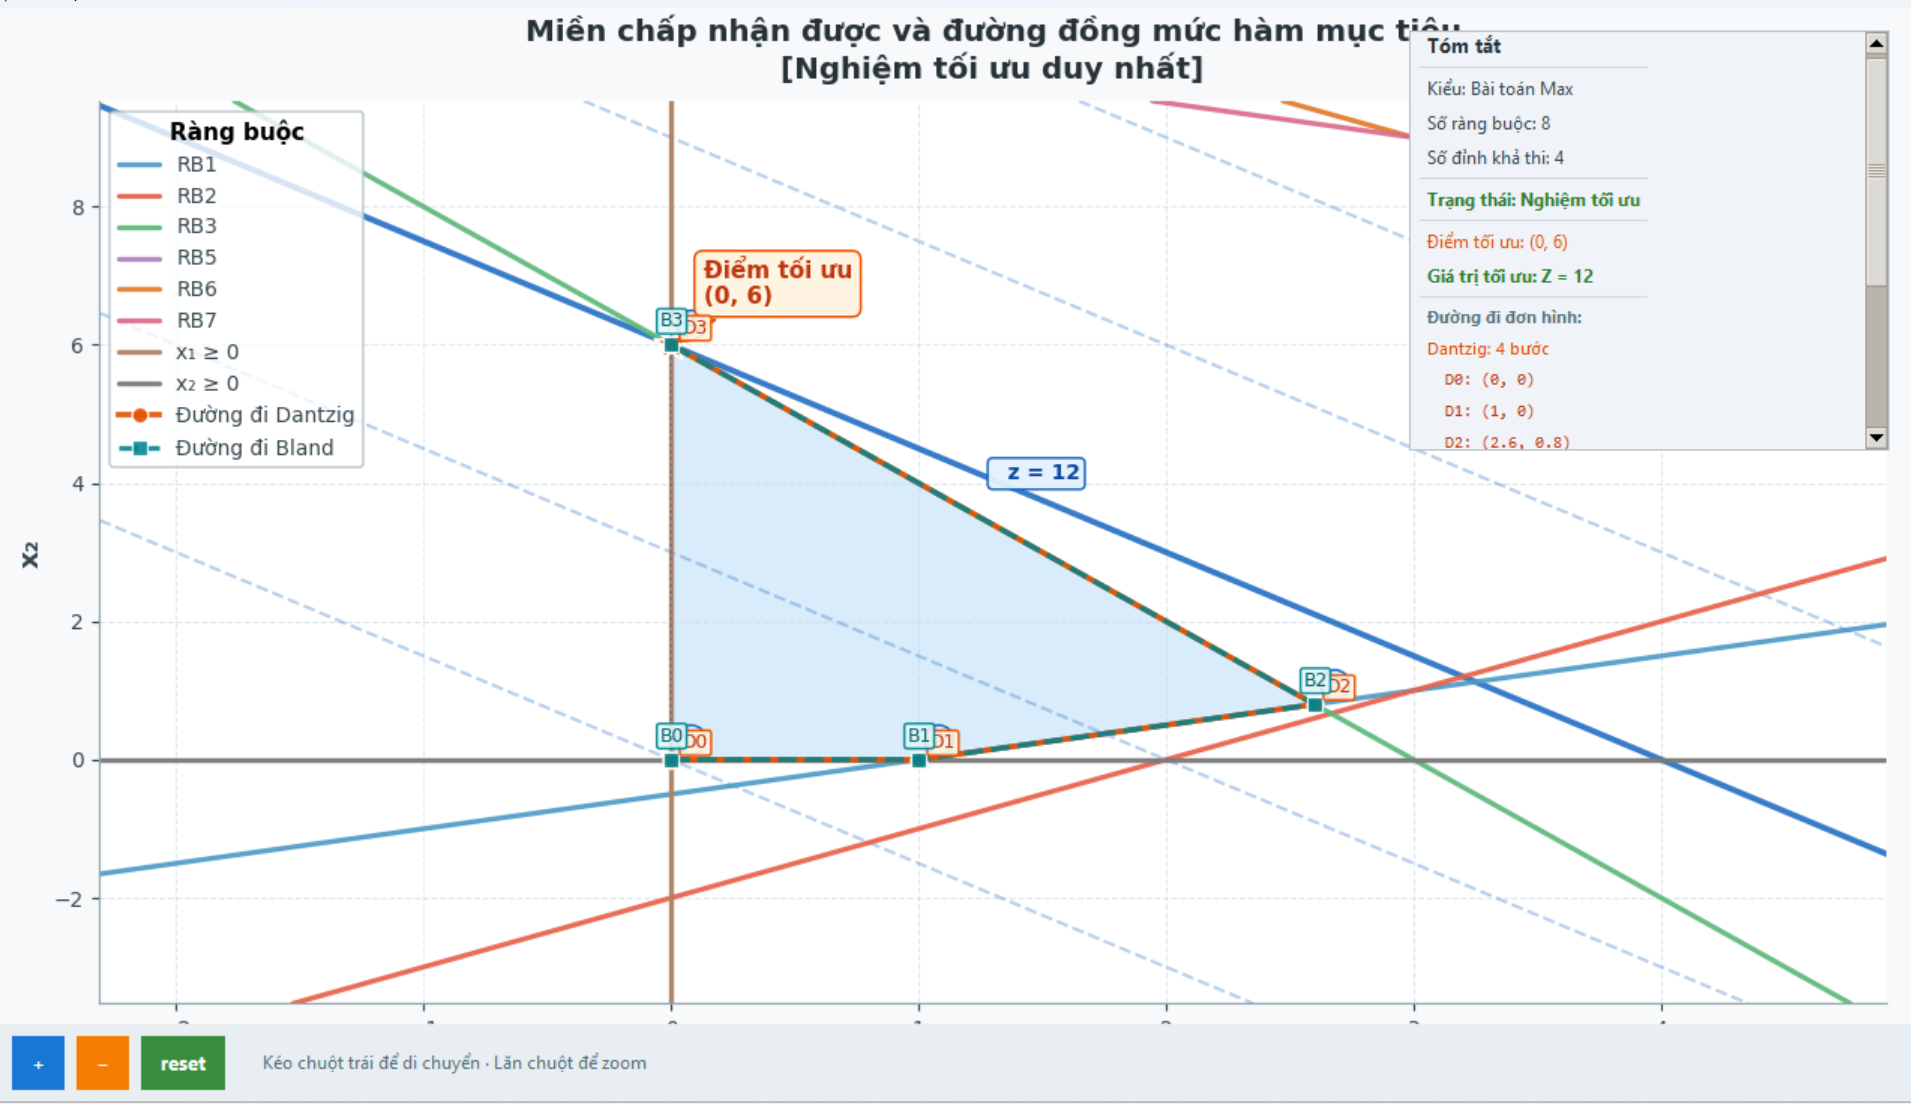
\includegraphics[width=0.75\textwidth]{Images/2D.png}
    \caption{Hình ảnh đồ thị 2D}
    \label{fig:buoc5s}
\end{figure}

\begin{figure}[H] %
    \centering
    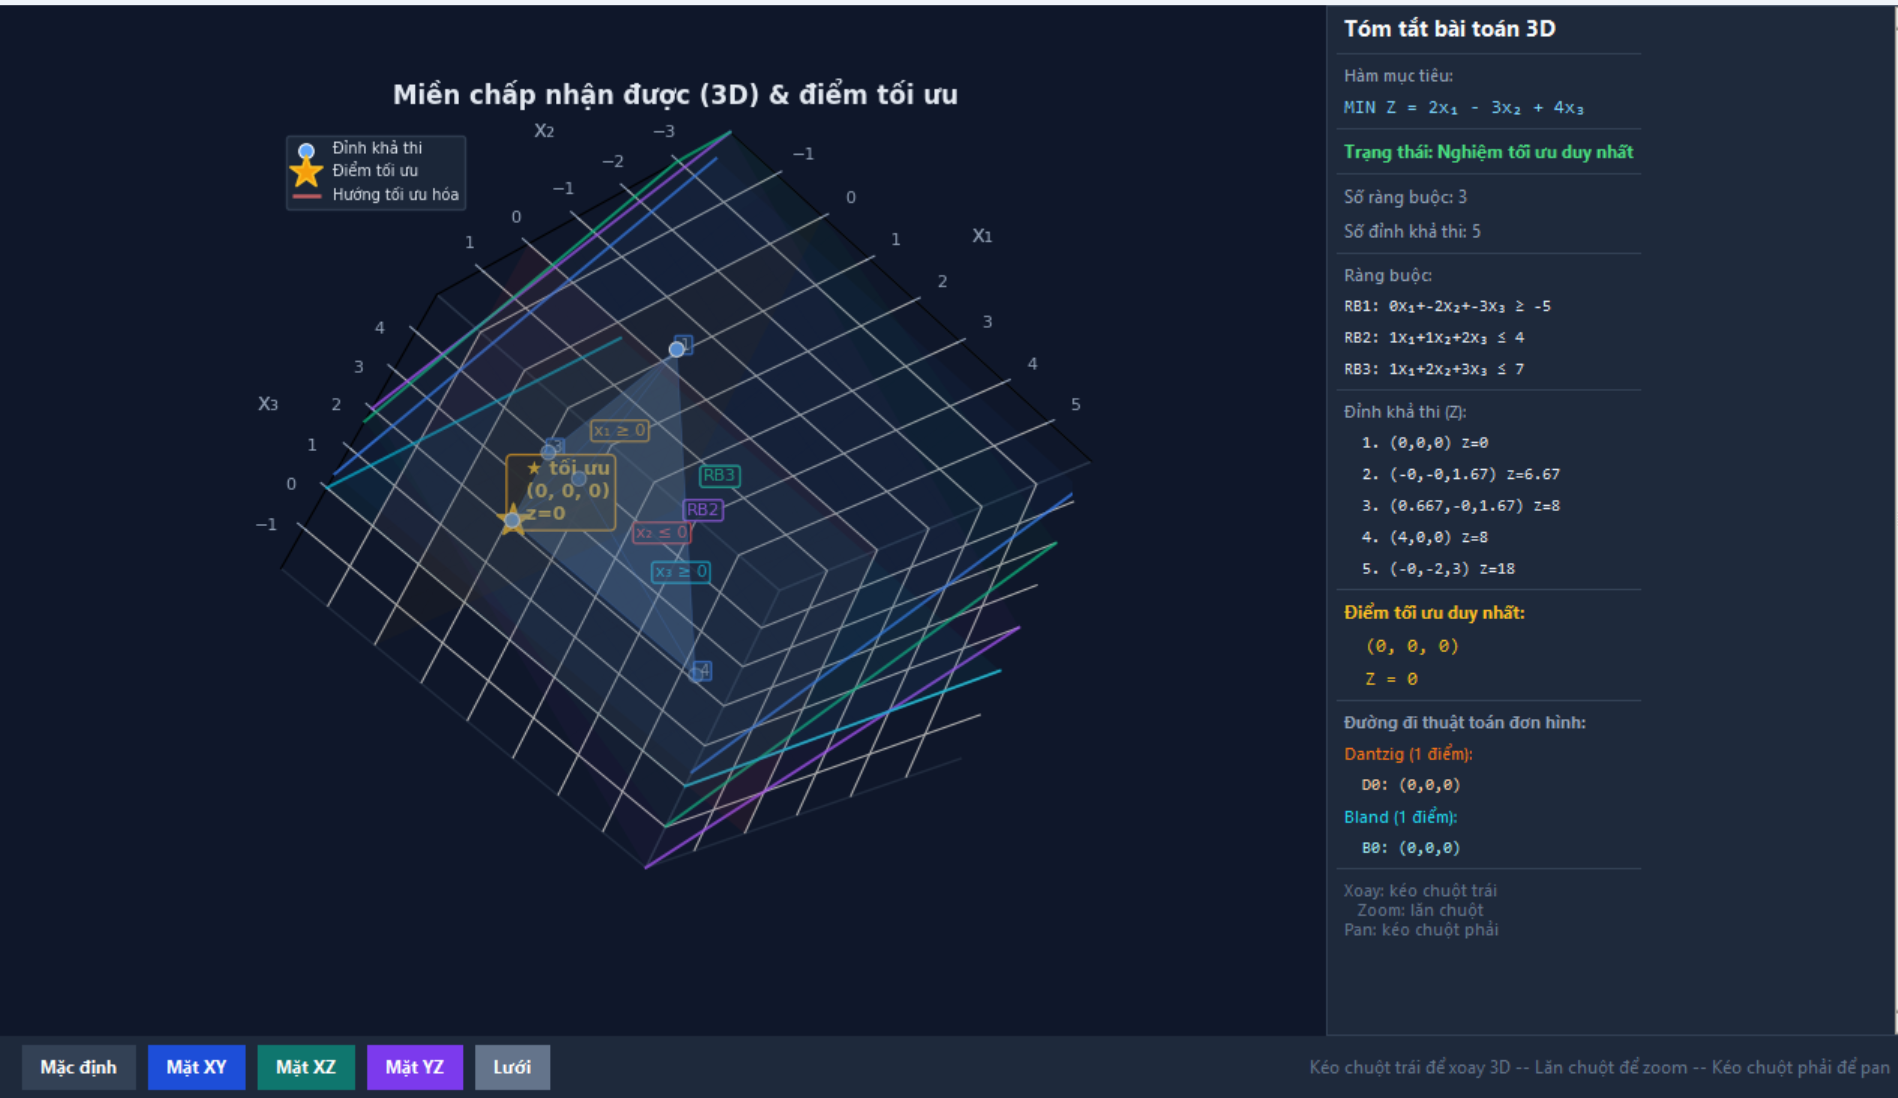
\includegraphics[width=0.75\textwidth]{Images/3D.png}
    \caption{Hình ảnh đồ thị 3D}
    \label{fig:buoc5ss}
\end{figure}


\newpage
\section{ĐÁNH GIÁ VÀ KẾT LUẬN}

\subsection{Các trường hợp đã xử lý thành công}
\textbf{Ứng dụng đã làm được:}
\begin{itemize}[label=\textcolor{secondary}{$\bullet$}, itemsep=1pt]
    \item Giải đúng và đầy đủ bốn trường hợp cơ bản của bài toán quy hoạch tuyến tính: tối ưu duy nhất, vô số nghiệm, không giới nội, vô nghiệm - cả khi không cần Pha 1 lẫn khi cần Pha 1 bổ trợ $x_0$.
    \item Giải thích rõ ràng từng bước: không chỉ đưa ra đáp án mà trình bày đầy đủ các bước chuẩn hóa bài toán, lý do sử dụng hai pha, lý do chọn biến vào/ra, bảng tỉ số $\theta$, phần tử xoay, ràng buộc của nghiệm trong trường hợp vô số nghiệm, lý do bài toán vô nghiệm hoặc không giới nội. Phù hợp để dùng trong lớp học.
    \item Chính xác tuyệt đối nhờ cho phép dùng kiểu dữ liệu Phân số - không có sai số làm tròn như các công cụ dùng số thực (float).
    \item Hỗ trợ nhập dữ liệu đa dạng: số nguyên, số thực, phân số.
    \item Phát hiện và xử lý xoay vòng.
    \item Trực quan hóa hình học đúng và đẹp cho bài 2 biến lẫn 3 biến, kể cả các trường hợp miền không bị chặn.
    \item Giao diện chuyên nghiệp: palette màu Nordic Frost nhất quán, hover effect, phím tắt, hỗ trợ cuộn chuột trong bảng nhập liệu lớn.
    \item Một số nút hoặc vùng chức năng chỉ khả dụng trong trường hợp người dùng nhấn \textbf{Chạy giải thuật} như: nút Xem HTML, Hiện từ vựng, Trực quan hóa và vùng Tham chiếu Phương pháp giải.
    \item Hỗ trợ đề xuất phương pháp giải phù hợp (có nêu lý do) và giải bằng cách khác đối với trường hợp Dantzig / Bland.
    \item Hiển thị HTML chất lượng cao: dùng KaTeX render công thức, có highlight bảng, tương thích nhiều trình duyệt.
    \item Chạy đa luồng: Dantzig và Bland chạy song song, cho phép hiển thị và so sánh ngay lập tức.
\end{itemize}

\subsection{Ưu điểm}
\begin{itemize}[label=\textcolor{secondary}{$\bullet$}, itemsep=1pt]
    \item Hiển thị toàn bộ quá trình chuẩn hóa (biến đổi tường minh từng ràng buộc và từng biến), không chỉ kết quả cuối. Định dạng HTML giúp bài toán được thể hiện một cách chuyên nghiệp nhất.
    \item Nghiệm tổng quát cho trường hợp vô số nghiệm: trình bày dạng tham số, tính khoảng giá trị hợp lệ của tham số.
    \item Animator - chức năng hiếm thấy ở các công cụ Quy hoach tuyến tính khác: phát lại từng bảng từ vựng như slideshow có màu sắc.
    \item Tự động đề xuất phương pháp dựa trên cấu trúc bài toán, kèm giải thích lý do.
    \item Tất cả trong một file thực thi: không cần kết nối mạng, không cần tài khoản, không có quảng cáo.
    \item Xây dựng luồng xử lý rõ ràng để dễ dàng tích hợp thêm các tính năng nâng cao trong tương lai.
    \item Việc có thể đối chiếu song song 2 phương pháp Bland và Dantzig giúp người dùng hiểu thêm về các cách tiếp cận khác nhau trong bài toán Quy hoạch tuyến tính.
\end{itemize}

\subsection{Hạn chế}
\textbf{Hạn chế về quy mô:}
\begin{itemize}[label=\textcolor{secondary}{$\bullet$}, itemsep=1pt]
    \item Số biến bị giới hạn tối đa 5, số ràng buộc tối đa 10. Bài toán thực tế (hàng chục/trăm biến) không giải được.
\end{itemize}

\medskip
\noindent\textbf{Hạn chế về thuật toán:}
\begin{itemize}[label=\textcolor{secondary}{$\bullet$}, itemsep=1pt]
    \item Còn thiếu thuật toán đối ngẫu (so với phạm vi kiến thức đã được học, tuy nhiên đã giải quyết được hết các trường hợp của bài toán quy hoạch tuyến tính).
    \item Trong Pha 1 bổ trợ, khi biến ra được chọn để xoay mà có nhiều hàng cùng tỉ số $\theta$ nhỏ nhất, phần mềm ưu tiên chọn hàng chứa $x_0$ nếu có. Lý do: nếu chọn $x_0$ ra khỏi cơ sở thì $\delta = x_0 = 0$, Pha 1 kết thúc và chuyển sang Pha 2. Ngược lại, nếu chọn một biến khác ra thay vì $x_0$ (dù vẫn hợp lệ về mặt toán học vì $x_0 = 0$), từ vựng tiếp theo có thể đã tối ưu theo hàm bổ trợ $\delta$ nhưng $x_0$ vẫn còn trong cơ sở với giá trị 0 - lúc đó thuật toán dễ kết luận nhầm là vô nghiệm.
\end{itemize}

\medskip
\noindent\textbf{Một số trường hợp xử lý chưa hoàn toàn trơn tru:}
\begin{itemize}[label=\textcolor{secondary}{$\bullet$}, itemsep=1pt]
    \item Trực quan hóa 3D còn hạn chế trong một số cấu hình miền khả thi phức tạp (nhiều mặt).
\end{itemize}

\subsection{Kết luận}
Dự án \textit{\textbf{“Phần mềm Giải bài toán Quy hoạch tuyến tính tổng quát”}} đã hoàn thành mục tiêu xây dựng một công cụ hỗ trợ học tập đắc lực cho sinh viên ngành Khoa học dữ liệu nói riêng và những người quan tâm đến lĩnh vực tối ưu hóa nói chung.

Thông qua quá trình thực hiện, nhóm đã đạt được những kết quả cụ thể:
\begin{itemize}[label=\textcolor{primary}{$\checkmark$}]
    \item \textbf{Về mặt kỹ thuật:} Xây dựng thành công một bộ giải mạnh mẽ, có khả năng xử lý bài toán đơn hình với đầy đủ các tình huống đặc biệt, đảm bảo tính chính xác và logic.
    \item \textbf{Về mặt ứng dụng:} Tích hợp thành công giao diện đồ họa thân thiện, hỗ trợ xuất báo cáo và trực quan hóa hình học 2D/3D – những tính năng giúp xóa bỏ rào cản giữa lý thuyết toán học trừu tượng và thực hành.
    \item \textbf{Về mặt kỹ năng:} Qua dự án, các thành viên trong nhóm đã rèn luyện được tư duy lập trình hệ thống, kỹ năng làm việc nhóm qua nền tảng Git/GitHub, cũng như khả năng phân tích và giải quyết vấn đề thực tế.
\end{itemize}

Mặc dù vẫn còn một ít hạn chế, phần mềm hiện tại đã đáp ứng tốt yêu cầu nghiên cứu và học tập. Trong tương lai, nhóm dự định sẽ tiếp tục phát triển thêm các tính năng như tối ưu hóa tốc độ xử lý, hỗ trợ bài toán quy mô lớn hơn, và cải thiện giao diện để nâng cao trải nghiệm người dùng.

Dự án không chỉ là một sản phẩm phần mềm, mà là minh chứng cho sự nỗ lực và tinh thần học hỏi của nhóm trong suốt quá trình thực hiện. Hy vọng sản phẩm này sẽ là tiền đề để nhóm tiếp tục phát triển các ứng dụng kỹ thuật phức tạp hơn trong tương lai.

\newpage
\section{MỘT SỐ PHẦN MỀM PHỔ BIẾN ĐỂ GIẢI BÀI TOÁN QUY HOẠCH TUYẾN TÍNH}
Để làm rõ vị thế của phần mềm nhóm, chúng em đã thực hiện khảo sát và so sánh với các công cụ giải bài toán Quy hoạch tuyến tính (QHTT) phổ biến hiện nay:

\subsection{PHPSimplex (Công cụ hỗ trợ học tập trực tuyến)}
Đây là công cụ điển hình phục vụ mục đích giảng dạy và học tập trực tuyến mà không cần cài đặt.

\medskip
\noindent\textbf{Cách sử dụng:}
\begin{itemize}[label=\textcolor{secondary}{$\circ$}]
    \item \textbf{Bước 1:} Truy cập trang web \url{phpsimplex.com}.
    \item \textbf{Bước 2:} Chọn số lượng biến và số lượng ràng buộc.
    \item \textbf{Bước 3:} Nhập các hệ số của hàm mục tiêu và các ràng buộc vào bảng biểu.
    \item \textbf{Bước 4:} Nhấn nút "Continue" để tiến hành giải. Hệ thống sẽ tự động chuyển bài toán sang dạng chuẩn và giải từng bước.
    \item \textbf{Bước 5:} Sử dụng nút "Next step" để xem các bước xoay của bảng đơn hình.
\end{itemize}
\textbf{Ưu điểm:} Cung cấp giao diện trực quan cho bài toán 2 biến (vẽ đồ thị). Đặc biệt hữu ích với bài toán nhiều biến nhờ khả năng hiển thị chi tiết từng bảng đơn hình (Simplex table), giúp người học đối chiếu các bước giải tay.\\
\textbf{Hạn chế:} Nhập liệu thủ công, thiếu tính linh hoạt khi làm việc với tập dữ liệu lớn và không hỗ trợ xử lý dữ liệu từ file bên ngoài.

\subsection{Microsoft Excel (Solver Add-in)}
Công cụ phổ biến trong môi trường văn phòng và phân tích kinh tế nhờ tính sẵn có và dễ dùng.

\medskip
\noindent\textbf{Cách sử dụng:}
\begin{itemize}[label=\textcolor{secondary}{$\circ$}]
    \item \textbf{Bước 1: Nhập liệu:} Nhập các hệ số của bài toán vào các ô trong bảng tính (Excel Sheet).
    \item \textbf{Bước 2: Thiết lập hàm mục tiêu:} Sử dụng hàm \texttt{=SUMPRODUCT()} để tính giá trị của hàm mục tiêu và các vế trái của ràng buộc.
    \item \textbf{Bước 3: Kích hoạt Solver:} Vào tab Data $\rightarrow$ chọn Solver.
    \item \textbf{Bước 4: Cấu hình:} 
    \begin{itemize}
        \item Đặt ô mục tiêu (Objective Cell).
        \item Chọn Max hoặc Min.
        \item Chọn các ô biến quyết định (Changing Variable Cells).
        \item Thêm các điều kiện ràng buộc (Constraints).
    \end{itemize}
    \item \textbf{Bước 5: Giải thuật:} Chọn phương thức Simplex LP và nhấn Solve để nhận nghiệm tối ưu.
\end{itemize}
\textbf{Ưu điểm:} Tích hợp sâu vào bảng tính, không yêu cầu kỹ năng lập trình. Solver cung cấp các báo cáo chuyên sâu như Độ nhạy (Sensitivity Report) và Giới hạn (Limits Report), rất hữu ích cho các bài toán ra quyết định kinh doanh.\\
\textbf{Hạn chế:} Mang tính "hộp đen", chỉ đưa ra kết quả cuối cùng mà không giải thích quá trình biến đổi của thuật toán, gây khó khăn cho việc nghiên cứu bản chất môn học. Ngoài ra, Solver bị giới hạn cứng về số lượng biến và ràng buộc trong bản tiêu chuẩn.

\subsection{Gurobi Optimizer (Trình tối ưu hóa công nghiệp)}
Đây là tiêu chuẩn vàng trong lĩnh vực tối ưu hóa thương mại, được các tập đoàn lớn tin dùng.

\medskip
\noindent\textbf{Cách sử dụng:}
\begin{itemize}[label=\textcolor{secondary}{$\circ$}]
    \item \textbf{Bước 1: Cài đặt:} Cần cài đặt thư viện Gurobi qua pip (\texttt{pip install gurobipy}) và đăng ký license (miễn phí cho mục đích học thuật).
    \item \textbf{Bước 2: Lập trình:} Người dùng phải viết mã nguồn (script) Python để định nghĩa mô hình:
    \begin{itemize}
        \item Khởi tạo \texttt{Model = gp.Model()}.
        \item Thêm các biến quyết định qua \texttt{Model.addVar()}.
        \item Thiết lập hàm mục tiêu qua \texttt{Model.setObjective()}.
        \item Thêm ràng buộc qua \texttt{Model.addConstr()}.
    \end{itemize}
    \item \textbf{Bước 3: Thực thi:} Gọi \texttt{Model.optimize()} để trình tối ưu hóa tự động tìm lời giải tối ưu.
    \item \textbf{Bước 4: Kết quả:} Truy xuất kết quả thông qua các thuộc tính của biến như X.
\end{itemize}
\textbf{Ưu điểm:} Sở hữu tốc độ xử lý vượt trội nhờ thuật toán Điểm trong (Interior Point) và khả năng xử lý song song, giải quyết được các bài toán có quy mô lên tới hàng triệu biến số. Gurobi hỗ trợ API mạnh mẽ cho nhiều ngôn ngữ lập trình như Python, C++.\\
\textbf{Hạn chế:} Không có giao diện nhập liệu đồ họa (người dùng phải lập trình), chi phí bản quyền thương mại rất cao, đòi hỏi chuyên môn kỹ thuật sâu mới có thể triển khai.

\vspace{0.5cm}
\begin{mdframed}[linecolor=secondary, linewidth=1.5pt, roundcorner=5pt, backgroundcolor=green!5]
    \textbf{$\rightarrow$ Điểm khác biệt của phần mềm này so với danh sách trên:} là công cụ duy nhất \textbf{miễn phí, chạy offline, hiển thị đầy đủ từng bước xoay có giải thích}, hỗ trợ tất cả dạng LP tổng quát (ràng buộc $\geq/=/\leq$, biến tự do/âm), tính toán chính xác với phân số, và có \textbf{animation từ vựng}.
\end{mdframed}

\newpage
\addcontentsline{toc}{section}{TÀI LIỆU THAM KHẢO}
\section*{TÀI LIỆU THAM KHẢO}
\begin{enumerate}
    \item Phan Quốc Khánh, Trần Tuệ Nương (2002). \textit{Giáo trình Quy hoạch tuyến tính}. Nhà xuất bản Đại học Quốc gia TP.HCM.
    \item Hillier, F. S., \& Lieberman, G. J. (2015). \textit{Introduction to Operations Research (10th Edition)}. McGraw-Hill Education. 
    \item Bazaraa, M. S., Jarvis, J. J., \& Sherali, H. D. (2011). \textit{Linear Programming and Network Flows}. Wiley. 
    \item Python Software Foundation. \textit{Tkinter - Python interface to Tcl/Tk}. Truy cập tại: \url{https://docs.python.org/3/library/tkinter.html}
    \item The Matplotlib Development Team. \textit{Matplotlib: Visualization with Python}. Truy cập tại: \url{https://matplotlib.org/stable/contents.html}
    \item GitHub. \textit{Linear Programming Tool Repository}. Nguồn mã nguồn dự án: \url{https://github.com/vngthdat206/LinearProgrammingTool_byVC}
    \item Vanderbei, R. J. (2014). \textit{Linear Programming: Foundations and Extensions (4th ed.)}. Springer.
    \item Bazaraa, M. S., Jarvis, J. J., \& Sherali, H. D. (2010). \textit{Linear Programming and Network Flows (4th ed.)}. Wiley.
    \item Bland, R. G. (1977). New finite pivoting rules for the simplex method. \textit{Mathematics of Operations Research}, 2(2), 103–107.
    \item Beale, E. M. L. (1955). Cycling in the dual simplex algorithm. \textit{Naval Research Logistics Quarterly}, 2(4), 269–275.
    \item Tài liệu Python chính thức: \textit{fractions.Fraction} - \url{https://docs.python.org/3/library/fractions.html}
    \item KaTeX - Thư viện render LaTeX cho HTML: \url{https://katex.org}
\end{enumerate}


\newpage
\addcontentsline{toc}{section}{PHỤ LỤC}
\section*{PHỤ LỤC: CÁC TEST CASE KIỂM THỬ MÔ HÌNH}

Dưới đây là các bộ kiểm thử (Test cases) tiêu biểu, bao phủ các kịch bản có thể xảy ra của bài toán Quy hoạch tuyến tính. Các bài toán này bao gồm cả những kịch bản đã được tích hợp sẵn mặc định trong ứng dụng và các kịch bản tùy chỉnh do người dùng nạp từ bên ngoài vào hệ thống.

\begin{tcolorbox}[colback=cyan!10!white, colframe=cyan!40!black, title=\textbf{Danh mục các bài toán mẫu tích hợp trong ứng dụng}, arc=1mm]
\begin{itemize}
    \setlength{\itemsep}{2pt}
    \item Ví dụ duy nhất nghiệm (Dantzig / Bland) \textit{hoặc} (hai pha)
    \item Ví dụ không giới nội (Dantzig / Bland) \textit{hoặc} (hai pha)
    \item Ví dụ vô số nghiệm (Dantzig / Bland) \textit{hoặc} (hai pha)
    \item Ví dụ vô nghiệm (hai pha)
    \item Ví dụ xoay vòng (Dantzig $\to$ Bland) \textit{hoặc} (hai pha $\to$ Dantzig $\to$ Bland)
\end{itemize}
Trong đó: có đầy đủ các trường hợp như bài toán $\max$, ràng buộc $\geq$, ràng buộc đẳng thức, biến tự do, biến không dương.
\end{tcolorbox}

\subsection*{TEST CASE 1: Bài toán nghiệm duy nhất (Dantzig / Bland)}
\noindent \textbf{a)} Bài toán trích xuất từ \colorbox{green!30}{Ví dụ duy nhất nghiệm (Dantzig / Bland)} có sẵn trong hệ thống:
\begin{equation*}
    \begin{aligned}
        \max z &= 3x_1 + 2x_2 \\
        \text{s.t.} \quad 
        &\begin{cases}
            -x_1 + 2x_2 \geq -1 \\
            x_1 - x_2 \leq 2 \\
            -2x_1 - x_2 \geq -6 \\
            x_1 \leq 5 \\
            2x_1 + x_2 \leq 16 \\
            x_1 + x_2 \leq 12 \\
            x_1 + 2x_2 \leq 21 \\
            x_2 \leq 10\\
            x_1, x_2 \geq 0
        \end{cases}
    \end{aligned}
\end{equation*}

Nghiệm tối ưu: $x_1^* = 0,\ x_2^* = 6$ và giá trị tối ưu $z^* = 12$.

\textit{Bài này kiểm tra xử lý bài toán $\max$ và ràng buộc $\geq$.}

\noindent \textbf{b)} Bài toán khác, có thể tải file \href{https://drive.google.com/uc?export=download&id=1i2pmndpwRcxOxdcEim4_M5tUnrq7TVHh}{\texttt{test\_case\_1.csv}} về:
\begin{equation*}
    \begin{aligned}
        \min z &= 2x_1 - 5x_2 \\
        \text{s.t.} \quad 
        &\begin{cases}
            x_1 + 3x_2 \leq 10 \\
            2x_1 - 3x_2 \leq 0 \\
            -x_1 + x_2 \leq 3 \\
            -x_1 + 2x_2 \leq 1
        \end{cases}
    \end{aligned}
\end{equation*}

Nghiệm tối ưu: $x_1^* = 3,\ x_2^* = 2$ và giá trị tối ưu $z^* = -4$.

\textit{Bài này kiểm tra xử lý biến tự do.\\Ngoài ra, từ vựng cuối xuất hiện $b_1, b_2$ với hệ số bằng $0$ trong hàm mục tiêu, thoạt nhìn như vô số nghiệm, nhưng vì $x_i = a_i - b_i$ nên nghiệm vẫn là duy nhất.}


\subsection*{TEST CASE 2: Bài toán nghiệm duy nhất (Hai pha)}

\noindent \textbf{a)} Bài toán trích xuất từ \colorbox{green!30}{Ví dụ duy nhất nghiệm (Hai pha)} có sẵn trong hệ thống:
\begin{equation*}
    \begin{aligned}
        \min z &= 5x_1 - 7x_2 \\
        \text{s.t.} \quad
        &\begin{cases}
            -4x_1 + x_2  \leq -2 \\
             x_1  + x_2  \leq  5 \\
            -x_1  - x_2  \leq -1 \\
            x_1, x_2 \geq 0
        \end{cases}
    \end{aligned}
\end{equation*}

Nghiệm tối ưu: $x_1^* = \dfrac{7}{5},\ x_2^* = \dfrac{18}{5}$ và giá trị tối ưu $z^* = -\dfrac{91}{5}$.

\textit{Bài này kiểm tra xử lý ràng buộc đẳng thức.}

\noindent \textbf{b)} Bài toán khác, có thể tải file \href{https://drive.google.com/uc?export=download&id=1O4QGTJxK5n-FU3EP5jCWbI_SLqUqUxHs}{\texttt{test\_case\_2.csv}} về:
\begin{equation*}
    \begin{aligned}
        \min z &= 2x_1 - x_2 + 2x_3 - x_4 + 4x_5 \\
        \text{s.t.} \quad
        &\begin{cases}
            4x_1 - 2x_2 + 13x_3 - 3x_4 + x_5 = 17 \\
            x_1  -  x_2 +  5x_3 -  x_4 + x_5 =  7 \\
            x_1, x_3, x_5 \geq 0,\quad x_2, x_4 \leq 0
        \end{cases}
    \end{aligned}
\end{equation*}

Nghiệm tối ưu: $x_1^* = 0,\ x_2^* = -2,\ x_3^* = 1,\ x_4^* = 0,\ x_5^* = 0$ và giá trị tối ưu $z^* = 4$.

\textit{Bài này kiểm tra xử lý biến $\geq 0$ và ràng buộc đẳng thức.}

\subsection*{TEST CASE 3: Bài toán không giới nội (Dantzig / Bland)}

\noindent \textbf{a)} Bài toán trích xuất từ \colorbox{green!30}{Ví dụ không giới nội (Dantzig / Bland)} có sẵn trong hệ thống:
\begin{equation*}
    \begin{aligned}
        \max z &= x_1 + x_2 \\
        \text{s.t.} \quad
        &\begin{cases}
            -x_1 + x_2 \leq 1 \\
             x_1 - 2x_2 \leq 2 \\
            x_1, x_2 \geq 0
        \end{cases}
    \end{aligned}
\end{equation*}

Kết luận: bài toán không giới nội ($z_{\max} = +\infty$) do tồn tại biến vào nhưng không có biến ra.

\textit{Bài này kiểm tra xử lý bài toán $\max$.}

\noindent \textbf{b)} Bài toán khác, có thể tải file \href{https://drive.google.com/uc?export=download&id=1bhEezs8vDbxG-h9YroT_dE6cqpEMrtwA}{\texttt{test\_case\_3.csv}} về:
\begin{equation*}
    \begin{aligned}
        \max z &= x_1 + 3x_2 - x_3 \\
        \text{s.t.} \quad
        &\begin{cases}
            2x_1 + 2x_2 - x_3 \leq 10 \\
            3x_1 - 2x_2 + x_3 \leq 10 \\
             x_1 - 3x_2 + x_3 \leq 10 \\
            x_1, x_2, x_3 \geq 0
        \end{cases}
    \end{aligned}
\end{equation*}

Kết luận: bài toán không giới nội ($z_{\max} = +\infty$) do tồn tại biến vào nhưng không có biến ra.

\textit{Bài này kiểm tra xử lý bài toán $\max$.}

\subsection*{TEST CASE 4: Bài toán không giới nội (Hai pha)}

\noindent \textbf{a)} Bài toán trích xuất từ \colorbox{green!30}{Ví dụ không giới nội (Hai pha)} có sẵn trong hệ thống:
\begin{equation*}
    \begin{aligned}
        \min z &= -2x_1 - x_2 \\
        \text{s.t.} \quad
        &\begin{cases}
            x_1 - x_2 \geq 1 \\
            x_1 + x_2 \geq 2 \\
            x_1, x_2 \geq 0
        \end{cases}
    \end{aligned}
\end{equation*}

Bài toán không giới nội ($z_{\max} = +\infty$) do tồn tại biến vào nhưng không có biến ra.

\textit{Bài này kiểm tra xử lý ràng buộc $\geq$.}

\noindent \textbf{b)} Bài toán khác, có thể tải file \href{https://drive.google.com/uc?export=download&id=1fs_9FGE6UBSGETVtR-QXNirOD6CHXkU0}{\texttt{test\_case\_4.csv}} về:
\begin{equation*}
    \begin{aligned}
        \min z &= 2x_1 - x_2 + 3x_3 + 7x_4 - 5x_5 \\
        \text{s.t.} \quad
        &\begin{cases}
            x_1 + 2x_2 +  x_3 + x_4 + 6x_5 \geq 10 \\
            2x_1 + 3x_2 + 4x_3 + x_4 + 2x_5 \geq  4 \\
            3x_1 + 2x_2 + 3x_4 + x_5 \leq  8 \\
            x_1, x_2 \geq 0,\quad x_3, x_4, x_5 \text{ tự do}
        \end{cases}
    \end{aligned}
\end{equation*}

Bài toán không giới nội ($z_{\min} = -\infty$) do tồn tại biến vào nhưng không có biến ra.

\textit{Bài này kiểm tra xử lý ràng buộc $\geq$ và biến tự do.}

\subsection*{TEST CASE 5: Bài toán vô số nghiệm (Dantzig / Bland)}

\noindent \textbf{a)} Bài toán trích xuất từ \colorbox{green!30}{Ví dụ vô số nghiệm (Dantzig / Bland)} có sẵn trong hệ thống:
\begin{equation*}
    \begin{aligned}
        \max z &= 2x_1 + 4x_2 \\
        \text{s.t.} \quad
        &\begin{cases}
            x_1 + 2x_2 \leq 6 \\
             x_1 \leq 4 \\
             x_2 \leq 3 \\
            x_1, x_2 \geq 0
        \end{cases}
    \end{aligned}
\end{equation*}

Nghiệm tối ưu: $\begin{cases}
    x_1 = x_1\\
    x_2 = 3 - \dfrac{1}{2}x_1
\end{cases}$, với $0 \leq x_1 \leq 4$ và giá trị tối ưu $z^* = 12$.

\textit{Bài này kiểm tra xử lý bài toán $\max$ và rút gọn điều kiện của 1 tham số.}

\noindent \textbf{b)} Bài toán khác, có thể tải file \href{https://drive.google.com/uc?export=download&id=1cSyDA359zQ8juj1aTRf-39mNglCkZVTj}{\texttt{test\_case\_5.csv}} về:
\begin{equation*}
    \begin{aligned}
        \max z &= x_1 + x_2 + x_3 \\
        \text{s.t.} \quad
        &\begin{cases}
            x_1 + x_2 + x_3 = 5 \\
            x_1 - x_2 + 3x_3 \leq 9 \\
            x_1, x_2, x_3 \geq 0
        \end{cases}
    \end{aligned}
\end{equation*}

Nghiệm tối ưu: $\begin{cases}
    x_1 = 5 - x_2 - x_3\\
    x_2 = x_2 \\
    x_3 = x_3
\end{cases}$, với $\begin{cases}
    - x_2 - x_3 \geq -5 \\
    2x_2 - 2x_3 \geq -4 \\
    x_2 \geq 0 \\
    x_3 \geq 0
\end{cases}$ và giá trị tối ưu $z^* = 5$.

\textit{Bài này kiểm tra xử lý bài toán $\max$, ràng buộc đẳng thức và rút gọn điều kiện của 2 tham số.}

\subsection*{TEST CASE 6: Bài toán vô số nghiệm (Hai pha)}

\noindent \textbf{a)} Bài toán trích xuất từ \colorbox{green!30}{Ví dụ vô số nghiệm (Hai pha)} có sẵn trong hệ thống:
\begin{equation*}
    \begin{aligned}
        \max z &= x_1 - x_2 \\
        \text{s.t.} \quad
        &\begin{cases}
            3x_1 + x_2 \geq 3 \\
            x_1 + 2x_2 \geq 4 \\
            x_1 - x_2 \leq 1 \\
            x_1 \leq 5 \\
            x_2 \leq 5 \\
            x_1, x_2 \text{ tự do}
        \end{cases}
    \end{aligned}
\end{equation*}

Nghiệm tối ưu: $\begin{cases}
    x_1 = 2 + \dfrac{1}{3}w_2\\
    x_2 = 1 + \dfrac{1}{3}w_2
\end{cases}$, với $0 \leq w_1 \leq 9$ và giá trị tối ưu $z^* = 1$.

\textit{Bài này kiểm tra xử lý bài toán $\max$, ràng buộc $\geq$, biến tự do và rút gọn điều kiện của 1 tham số.}

\noindent \textbf{b)} Bài toán là biến thể của bài toán trên (loại bỏ đi một số điều kiện):
\begin{equation*}
    \begin{aligned}
        \max z &= x_1 - x_2 \\
        \text{s.t.} \quad
        &\begin{cases}
            x_1 - x_2 \leq 1 \\
            x_1 \leq 5 \\
            x_2 \leq 5 \\
            x_1, x_2 \text{ tự do}
        \end{cases}
    \end{aligned}
\end{equation*}

Nghiệm tối ưu: $\begin{cases}
    x_1 = 1 + x_1\\
    x_2 = x_2
\end{cases}$, với $x_2 \leq 4$ và giá trị tối ưu $z^* = 1$.

Bài này có 1 ràng buộc $a_1 = 1 + b_1 + a_2 - b_2$ phải xử lý cả $\left(a_1, b_1\right)$ và $\left(a_1, b_1\right)$ (để suy ra $x_1 = 1 + x_2$) trong cùng một ràng buộc, trong khi bài toán trên chỉ phải xử lý một cặp ở từng ràng buộc $a_2 = 1 + b_2 + \dfrac{1}{3}w_2 \Rightarrow x_2 = 1 + \dfrac{1}{3}w_2$ và $a_1 = 2 + b_1 + \dfrac{1}{3}w_2\Rightarrow x_1 = 2 + \dfrac{1}{3}w_2$.

\noindent \textbf{b)} Bài toán khác, có thể tải file \href{https://drive.google.com/uc?export=download&id=1VtHEzV92zsS2A81G4-6bB8Fz9xFa4D6U}{\texttt{test\_case\_6.csv}} về:
\begin{equation*}
    \begin{aligned}
        \max z &= 4x_1 + 2x_2 - x_3 \\
        \text{s.t.} \quad
        &\begin{cases}
            -8x_1 - 2x_2 +  x_3 \geq 5 \\
            x_1 - 2x_2 \leq  3 \\
            3x_1 + -5x_3 \leq  9 \\
            x_1, x_2, x_3 \geq 0
        \end{cases}
    \end{aligned}
\end{equation*}

Nghiệm tối ưu: $\begin{cases}
    x_1 = 0\\
    x_2 = x_2\\
    x_3 = 5 + 2x_2
\end{cases}$, với $x_2 \geq 0$ và giá trị tối ưu $z^* = -5$.

\textit{Bài này kiểm tra xử lý bài toán $\max$, ràng buộc $\geq$ và rút gọn điều kiện của 1 tham số.}

\subsection*{TEST CASE 7: Bài toán vô nghiệm (Hai pha)}

\noindent \textbf{a)} Bài toán trích xuất từ \colorbox{green!30}{Ví dụ vô nghiệm (Hai pha)} có sẵn trong hệ thống:
\begin{equation*}
    \begin{aligned}
        \min z &= x_1 + x_2 \\
        \text{s.t.} \quad
        &\begin{cases}
            x_1 + 2x_2 \geq 2 \\
            3x_1 + 2x_2 \leq 1 \\
            x_1 + x_2 \geq 1 \\
            x_1, x_2 \geq 0
        \end{cases}
    \end{aligned}
\end{equation*}

Bài toán vô số nghiệm ($x_{\min} = + \infty$) vì $x_0$ còn trong cơ sở sau pha 1 (miền chấp nhận được rỗng).

\textit{Bài này kiểm tra xử lý ràng buộc $\geq$.}

\noindent \textbf{b)} Bài toán khác, có thể tải file \href{https://drive.google.com/uc?export=download&id=19AbIuvdUcsyOVT9u4zPvYWzQ_VboDXlr}{\texttt{test\_case\_7.csv}} về:
\begin{equation*}
    \begin{aligned}
        \min z &= 9x_1 - 8x_2 \\
        \text{s.t.} \quad
        &\begin{cases}
            x_1 + 2x_2 \leq 3 \\
            3x_1 + 4x_2 \geq 5 \\
            6x_1 + 7x_3 = 8 \\
            x_1 \geq 0, x_2 \leq 0
        \end{cases}
    \end{aligned}
\end{equation*}

Bài toán vô số nghiệm ($x_{\min} = + \infty$) vì $x_0$ còn trong cơ sở sau pha 1 (miền chấp nhận được rỗng).

\textit{Bài này kiểm tra xử lý ràng buộc $\geq$, ràng buộc đẳng thức, biến $\leq 0$.}

\subsection*{TEST CASE 8: Hiện tượng xoay vòng}

\noindent \textbf{a)} Bài toán trích xuất từ \colorbox{green!30}{Ví dụ xoay vòng (Dantzig $\rightarrow$ Bland)} có sẵn trong hệ thống:
\begin{align*}
    \min z &= -10x_1 + 57x_2 + 9x_3 + 24x_4 \\
    \text{s.t.} \quad 
    &\begin{cases}
        \dfrac{1}{2}x_1 - \dfrac{11}{2}x_2 - \dfrac{5}{2}x_3 + 9x_4 \leq 0 \\
        \dfrac{1}{2}x_1 - \dfrac{3}{2}x_2 - \dfrac{1}{2}x_3 + x_4 \leq 0 \\
        x_1 \leq 1 \\
        x_1, x_2, x_3, x_4 \geq 0
    \end{cases}
\end{align*}

\textit{Bài này kiểm tra phương pháp Bland giải quyết được trong khi phương pháp Dantzig thì không thể giải (xoay vòng lặp lại sau 6 bước).}

\noindent \textbf{b)} Bài toán trích xuất từ \colorbox{green!30}{Ví dụ xoay vòng (Hai pha $\rightarrow$ Dantzig $\rightarrow$ Bland)} có sẵn trong hệ thống:
\begin{align*}
    \min z &= \dfrac{3}{4}x_1 - 20x_2 + \dfrac{1}{2}x_3 - 6x_4 \\
    \text{s.t.} \quad 
    &\begin{cases}
        \dfrac{1}{4}x_1 - 8x_2 - x_3 + 9x_4 \leq 0 \\
        \dfrac{1}{2}x_1 - 12x_2 - \dfrac{1}{2}x_3 + 3x_4 \leq 0 \\
        -x_5 \leq -1 \\
        x_1, x_2, x_3, x_4, x_5 \geq 0
    \end{cases}
\end{align*}

\textit{Bài này kiểm tra phương pháp Bland giải quyết được trong khi phương pháp Dantzig thì không thể giải (Pha 2 xoay vòng lặp lại sau 6 bước).}



\end{document}